\documentclass[a4paper,10pt]{article}
\usepackage{amssymb}
\usepackage{alltt}\tiny
\usepackage{amsmath,amsfonts}
\usepackage{amsthm}
\usepackage{graphicx}
\usepackage{hyperref}
\usepackage{epstopdf}
\DeclareGraphicsExtensions{.pdf,.png,.jpg}
\newtheorem{theorem}{Theorem}[section]
\newtheorem{definition}[theorem]{Definition}
\newtheorem{lemma}[theorem]{Lemma}
\newcommand{\nop}[1]{}

% These are from candidacy edic.tex
\graphicspath{{./graphics/}}
\DeclareGraphicsExtensions{.pdf,.jpeg,.png}

% Legacy from Christoph's paper:
% \DeclareGraphicsRule{.tif}{png}{.png}{`convert #1 `dirname #1`/`basename #1 .tif`.png}

% When converting eps to pdf, suffix is added to filename. 
% Recommended not to be empty string by http://www.tex.ac.uk/tex-archive/macros/latex/contrib/oberdiek/epstopdf.pdf : page 4, suffix paragraph.
\epstopdfsetup{suffix=-generated}

\begin{document}

\title{Squall/Storm Quick Start Guide}
\date{}
\maketitle

\section{Introduction}
The document is organized as follows. Chapter~\ref{ch:perspective} discusses challenges in online processing and on very high level explains a system we are going to use. Chapter~\ref{ch:implementation} give more insights about the existing code, and Chapter~\ref{ch:installation} is an installation tutorial. Last chapter explains installation and use of our SQL plugin.

\section{A perspective from 10,000 feet}
\label{ch:perspective}
\vspace{2mm}
\textit{Squall} is an online query processing tool built on top of Storm (\url{https://github.com/nathanmarz/storm}). ``Online`` means that the final result is constantly updated as new tuples arrive into the system, and at each step the system represents an \emph{eventually} correct final result of the tuples seen so far. In contrast to batch processing, all the components are active all the time. In other words, there is no stage that waits for the completion of it precursor stage. \textit{Storm} is an online processing system, allowing a user to specify logical components and their allocation and interconnection in the cluster. A logical component might be executed on multiple physical nodes. Thus, by executing the same code on multiple physical nodes, data parallelism is achieved. Two logical components can be interconnected by an arbitrary function (e.g. by a hash function of some field in a tuple). In Storm terminology, these interconnection are called \textit{stream groupings}. Stream groupings offer more flexibility than the corresponding ones in Online MapReduce \cite{HopSigmod2010}. Specifically, Storm offers the user the possibility to reason about his system in terms of a DAG of components that contain arbitrary code and can be arbitrarily interconnected. A DAG of these logical components submitted to a parallel execution environment is denoted as a \textit{topology}. A topology is executed indefinitely, until a user explicitly kills it.

Squall uses Storm as its underlying parallel environment, and builds query operators on top of it. Squall is a Java program which use Storm's Java libraries. Squall transforms a query plan, consisting of a DAG of \emph{query operator} components, into a Storm topology. Currently, we have implemented a heuristic-based optimizer which generates bushy plans.

The following operators are supported: Selection, Projection, Distinct, Aggregation (Sum, Count and Average) and Join. All the operators have the expected semantics. Selection and Projection work ``on-the-fly'', as soon as a tuple arrives it is processed. Distinct and Aggregation operators need to store a state that is constantly updated. Each operator can be executed on a separate logical component, but inside a single logical component we can also pipeline the output of one operator to the input of another. The class \verb#ChainOperator# is responsible for this. The Join operator supports arbitrary equijoins and it works as follows: tuples with the same key have to be processed within a single node. Thus, it is guaranteed that the Join operator nodes will not have to communicate in order to produce the result. When a tuple arrives on a node, it is appended to the materialization of the corresponding relation and joined with the materialization of the opposite relation. For equijoins, it is quite efficient, since materializations are stored as hash tables containing join condition value as the key. This algorithm is essentially a version of Hash Ripple Join(~\cite{RippleJoin}) executing concurrently at multiple nodes. Our version of Hash Ripple Join provide a correct result for tuples seen so far (tuples which fully propagated). In contrast to its traditional counterpart, our version does not do sampling of the input tuples, yet it processes them as they arrive.

Note that Squall/Storm is not a production system - it works, but it is still in a beta stage. On this \href{http://groups.google.com/group/storm-user/browse_thread/thread/d4a50cf051ea878d/3c42dd8614aaf549?#3c42dd8614aaf549}{link}, the author of Storm admits that a topology fails with no valid reason once in every 50 runs. So, if you encounter a problem, try to execute the topology several times. If the problem persists, send us the complete source code you are using, the config file, and a full trace of the occurred Exception.

%A query component might consists of multiple Storm logical components.

\section{Some implementation details}
\label{ch:implementation}
\vspace{2mm}
In the Storm terminology, a logical component which generates tuples (or reads from a file) and propagates them further down the system, is called Spout, and all other components are denoted as Bolts. A Spout contains the \verb|nextTuple| method, which sends tuples down the topology, and Bolt contains \verb|execute(Tuple)| method which processes a tuple and/or sends it further down. 

From the Storm documentation:
\textit{Each spout or bolt executes as many tasks across the cluster. Each task corresponds to one thread of execution, and stream groupings define how to send tuples from one set of tasks to another set of tasks.}

However, each task executes sequentially - that is, \verb|nextTuple| or \verb|execute(Tuple)| are not called, until the processing of the previous tuple is done. You can set the parallelism for each component using the config files that we will explain later, as well as the total number of workers allocated. 

From the Storm documentation:
\textit{Topologies execute across one or more worker processes. Each worker process is a physical JVM and executes a subset of all the tasks for the topology. For example, if the combined parallelism of the topology is 300 and 50 workers are allocated, then each worker will execute 6 tasks (as threads within the worker). Storm tries to spread the tasks evenly across all the workers.}

Storm, by default, writes the final result nowhere, but we override this in Squall so that the last component prints the result by default. Where this result is stored depends on the Mode you are running Squall in (more details in the next section).

\section{Installation}
\label{ch:installation}
\vspace{2mm}
This section is a tutorial for installing Squall/Storm on your local machine, and for invoking it properly on the cluster, where it is already installed.

The following steps are necessary for both modes:
\begin{enumerate}
 \item Put the content of \verb#install# directory (not the directory itself) somewhere on your local machine. The directory where you put it will be denoted as \verb#INSTALL_DIR#. \verb#INSTALL_DIR# now contains 5 directories inside (auxiliary, bin, compilation, dip and lib). \textit{Do not change directory structure. Otherwise scripts for installation/running would not work!}
 \item Download Storm 0.7.0 from \url{https://github.com/nathanmarz/storm/downloads}, extract it, and put \verb#storm-0.7.0# directory in \verb#INSTALL_DIR#. Please note that you \textit{have to} use this version of Storm in order for Squall to run.
 
\subsection{Quick Start: Local Mode}
You will run Squall on TPCH database. The paths for TPCH databases for Cluster Mode are already set, but in Local Mode you need to set them up. Go to \verb#INSTALL_DIR/dip/Squall/confs/0.1G_hyracks_serial# and change \verb#DIP_DATA_PATH# such that it is a full path to a 0.1-scaling factor TPCH database on your local machine. If on your local machine you neither have DBGen installed, nor TPCH databases for scaling factors 0.1, you can \verb#scp# it from icdatasrv1 at the following location: \\ \verb#/export/home/avitorovic/queries/tpch/0.1G#. Inside \\ \verb#/export/home/avitorovic/queries/tpch/# remote directory you can find TPCH databases of different sizes as well (1G, 2G, 4G, 6G, 8G and 10G). For now, you will need only the one with scaling factor 0.1.

As usual, testing code in local mode is way better than in a cluster environment. Namely, in local mode all the errors go to the standard output/error, whereas in cluster mode one has to search for errors across many nodes. The same holds for presenting the final result.

You can run Squall in Local Mode by:
\begin{verbatim}
 cd $INSTALL_DIR/bin
 ./squallLocalRun.sh
\end{verbatim}
\end{enumerate}

Now we will talk about an output of a Squall/Storm run. In Local mode, all the output goes to console. First, Storm produces some output. You can safely ignore messages of the form \verb#Task 0.1G_hyracks_serial-1-1333023576:1 timed out#. This kind of messages always occurs when a task is started.

Then you will see something like:
\begin{verbatim}
... TopologyKiller: Received EOF message from: 2
... TopologyKiller: 1 remaining
... TopologyKiller: Received EOF message from: 3
... TopologyKiller: 0 remaining
... TopologyKiller: Received EOF from all spouts. Killing cluster...
\end{verbatim}

This shows the information about Spouts that have finished processing their input. When all Spouts are done, Squall/Storm produces the final result. In this case, it is:
\begin{verbatim}
The result for topology 0.1G_hyracks_serial
Component COUNTAGG:
Iteration 150000:
FURNITURE = 29074
BUILDING = 31264
MACHINERY = 30341
HOUSEHOLD = 29462
AUTOMOBILE = 29859
\end{verbatim}

\verb#Iteration# refers to the number of tuples the last component (named COUNTAGG) received.

Finally, you will encounter the lines containing the \verb#Async loop interrupted# message. You can safely ignore this, these messages appear when tasks are killed. At this point, your program is done. Since Storm is designed to execute forever, the process will block, so you have to stop it explicitly (for example CTRL+C in command line).

\subsection{Recompilation: both Local and Cluster Mode}
In order to recompile the code, you need to have Internet access on your local machine, due to the fact that some libraries are downloaded from web repositories. Our compilation procedure uses \verb#Leiningen# and \verb#maven2#, tools akin to \verb#make#. \verb#Leiningen# is available in \verb#INSTALL_DIR/bin/lein#, more information about the tool can be found at \url{https://github.com/technomancy/leiningen}. You need to install \verb#maven2# , for example from \url{http://maven.apache.org/download.html}. The reason why we use these tools is that they enable us to generate a single jar not only with source code, but also with third-party libraries. This is necessary in Cluster Mode, where we have to submit a single jar with all the non-Storm dependencies in the bundle.

The source code you are going to extend is available in \verb#INSTALL_DIR/dip/Squall/src#. You can add any package/class in this directory, and it will be compiled by the following commands:
\begin{verbatim}
 cd $INSTALL_DIR/bin
 ./recompile.sh
\end{verbatim}
The output of this command is a jar file: \\ \verb#INSTALL_DIR/compilation/squall-2.0-standalone.jar# (it will overwrite the old version of the same jar). You can run the modified code exactly the same as before.

After you run \verb#recompile.sh# for the first time, you do not need Internet access to download packages - they will be already in place. Thus, you can safely comment out the following lines from \verb#recompile.sh#:
\begin{verbatim}
 mvn install:install-file -DgroupId=jsqlparser -DartifactId=jsqlparser \
      -Dversion=0.7.0 -Dpackaging=jar -Dfile=../lib/jsqlparser-0.7.0.jar
../bin/lein clean
../bin/lein deps
\end{verbatim}

Alternatively, you can create a Java project in your favorite Java environment (Eclipse, NetBeans, ...), import the source code from \verb#INSTALL_DIR/dip/Squall/src#, reference to the following set of jars (exactly in this order):
\begin{enumerate}
 \item all the jar files inside \verb#INSTALL_DIR/storm-0.7.0/lib/#
 \item \verb#INSTALL_DIR/storm-0.7.0/storm-0.7.0.jar#
\end{enumerate}
and run Squall directly from a Java environment (do not use \verb#squallLocalRun.sh#!). In addition, you have to specify \verb#main.Main# as the main class, and the only argument is the config file full path. 

If you use third-party libraries (as we do in SQLplugin, which we explain later), and run your code in Cluster Mode, \textit{you would not be able to run Squall directly from your Java environment}. This is due to the fact that your Java environment would not create a single jar file with all non-Storm dependencies. In that case, you have to use \verb#squallClusterRun.sh#, which uses \verb#/squall-2.0-standalone.jar#.

\subsection{Query Plans and config files: Local Mode}
The script for running Squall in Local Mode is \verb#bin/squallLocalRun.sh# (ignore \verb#pluginSQLLocalRun.sh# for now). As you can see in \verb#bin/squallLocalRun.sh#, there is a parameter specifying a path to \textit{config file}. Config file describes which query plan from a set of predefined ones is going to be used, along with some other parameters we explain later in this document. Your config file has to be in \verb#INSTALL_DIR/dip/Squall/confs#, and as you can see from \verb#bin/squallLocalRun.sh#, \verb#0.1G_hyracks_serial# config file is used by default. 

In order to run Squall in Local Mode with some other config file, \textit{must set} \verb#DIP_DATA_PATH# for that config file such that it points to a database of the appropriate size on your machine and then run the following commands:
\begin{verbatim}
 cd $INSTALL_DIR/bin
 ./squallLocalRun.sh $CONFIG_FILE
\end{verbatim}
where \verb#CONFIG_FILE# is a file from \verb#INSTALL_DIR/dip/Squall/confs# which ends up with \verb#_serial#. If you do not want to use scripts, you can, for example, run the following commands:
\begin{verbatim}
 cd $INSTALL_DIR/bin
 java -cp ../compilation/squall-2.0-standalone.jar:../storm-0.7.0/lib/*:
          ../storm-0.7.0/storm-0.7.0.jar 
          main.Main ../dip/Squall/confs/0.1G_hyracks_serial
\end{verbatim}

As we already saw, by default, \verb#0.1G_hyracks_serial# config file is used. Now, we are going to give more details about what a config file represents. The config file refers to \verb#queryPlans.HyracksPlan# from the source code. The corresponding SQL query is as follows:
\begin{verbatim}
SELECT C_MKTSEGMENT, COUNT(O_ORDERKEY)
FROM CUSTOMER join ORDERS on C_CUSTKEY = O_CUSTKEY
GROUP BY C_MKTSEGMENT
\end{verbatim}

The reason why we call this plan Hyracks is because this is a SQL query appearing in the Hyracks paper (~\cite{Hyracks}). You do not need to read this paper.

However, Squall requires a query plan at the input, not SQL. For the SQL query we showed above, the corresponding query plan is presented below (this is actually a part of \verb#INSTALL_DIR/dip/Squall/src/queryPlans/HyracksPlan# class):
\begin{verbatim}
ProjectionOperator projectionCustomer = 
			new ProjectionOperator(new int[]{0, 6});
ArrayList<Integer> hashCustomer = 
			new ArrayList<Integer>(Arrays.asList(0));
DataSourceComponent relationCustomer = new DataSourceComponent(
                        "CUSTOMER",
                        dataPath + "customer" + extension,
                        TPCH_Schema.customer,
                        _queryPlan).setProjection(projectionCustomer)
                                   .setHashIndexes(hashCustomer);
//--------------------------------------------------------------------
ProjectionOperator projectionOrders = 
                        new ProjectionOperator(new int[]{1});
ArrayList<Integer> hashOrders = 
                        new ArrayList<Integer>(Arrays.asList(0));
DataSourceComponent relationOrders = 
                        new DataSourceComponent(
                          "ORDERS",
                          dataPath + "orders" + extension,
                          TPCH_Schema.orders,
                          _queryPlan).setProjection(projectionOrders)
                                    .setHashIndexes(hashOrders);                             
//--------------------------------------------------------------------
ArrayList<Integer> hashIndexes = new ArrayList<Integer>(Arrays.asList(1));
JoinComponent CUSTOMER_ORDERSjoin = new JoinComponent(
                    relationCustomer,
                    relationOrders,
                    _queryPlan).setHashIndexes(hashIndexes);

//--------------------------------------------------------------------
AggregateCountOperator agg = new AggregateCountOperator()
			         .setGroupByColumns(Arrays.asList(1));

OperatorComponent oc = 
       new OperatorComponent(CUSTOMER_ORDERSjoin, "COUNTAGG", _queryPlan)
                                        .setAggregation(agg);
\end{verbatim}

The explanation is provided in Figure~\ref{fig:Hyracks}. Note that we do not have to perform any projections on the \verb#CUSTOMER_ORDERS# join component. The output tuple does not contain \verb#CUSTKEY# from the right parent, since it is already included (with the same value) from the left parent. A hash from a parent relation (CUSTOMER, ORDERS) refers to a position(s) in a tuple \textit{after} projection is performed. The hash denotes the columns from a tuple that are join keys in the join component. You can find more query plan examples in the package \verb#queryPlans#. Their corresponding config files can be found in \verb#INSTALL_DIR/dip/Squall/confs#.

\begin{figure}
\centering
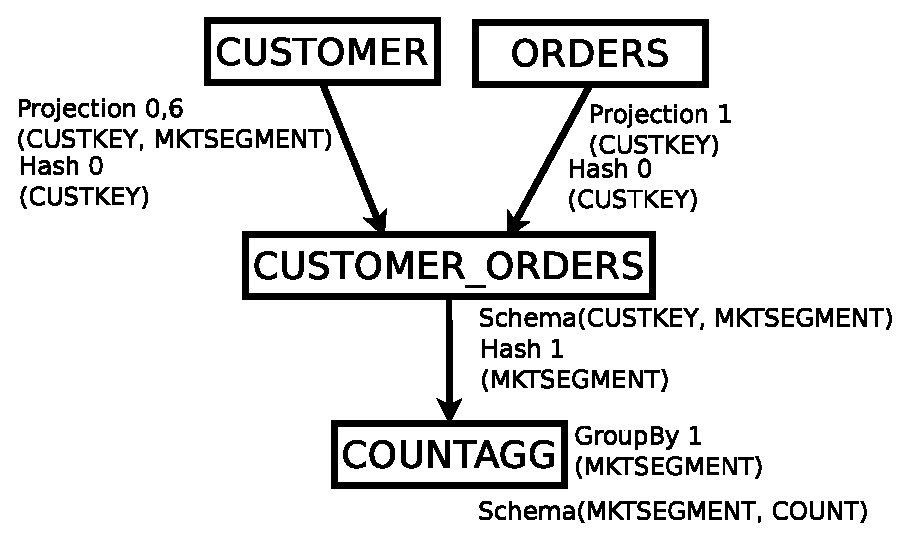
\includegraphics[width=4in]{Hyracks.eps}
\vspace{-3mm}
\caption{A query plan for the Hyracks query.}
\label{fig:Hyracks}
\vspace{-2mm}
\end{figure}

Now we discuss parameters inside a config file. Once more, we will use \verb#0.1G_hyracks_serial# for illustration:
\newpage
\begin{verbatim}
DIP_DISTRIBUTED false
DIP_QUERY_NAME hyracks
DIP_TOPOLOGY_NAME_PREFIX teamX
DIP_TOPOLOGY_NAME 0.1G_hyracks_serial
DIP_NUM_PARALLELISM 5
DIP_NUM_ACKERS 1

DIP_DATA_PATH /path/to/tpch0.1G/on/local/machine/

CUSTOMER_PAR 1
ORDERS_PAR 1

CUSTOMER_ORDERS_PAR 1
COUNTAGG_PAR 1

# below are unlikely to change
DIP_EXTENSION .tbl
DIP_READ_SPLIT_DELIMITER \|
DIP_GLOBAL_ADD_DELIMITER |
DIP_GLOBAL_SPLIT_DELIMITER \|

DIP_KILL_AT_THE_END true
#used only in distributed mode
DIP_NIMBUS_HOST icdatasrv2
DIP_STORM_ZOOKEEPER_SERVERS icdatasrv2
\end{verbatim}

\verb|DIP_DISTRIBUTED| must be false to execute the query plan in Local mode. \verb|DIP_QUERY_NAME| must be case-insensitive equal to a query plan from \verb#queryPlans# package, without the ``Plan'' suffix at the end. For example, here we have a query named ``hyracks'' which targets \verb#HyracksPlan# class. Topology name is built by concatenation of \verb#DIP_TOPOLOGY_NAME_PREFIX# and \verb|DIP_TOPOLOGY_NAME|. \\ \verb#DIP_TOPOLOGY_NAME_PREFIX# is there to distinguish different users, but it must be set only in Cluster Mode. In Local mode, \verb|DIP_NUM_PARALLELISM| refers to the number of threads allocated for Squall. As already mentioned, if your topology requires more tasks than are available through this parameter, some of the tasks will be collocated in a single thread. This setting is quite important, because if too many threads are instantiated, the execution will be very slow. \verb|DIP_NUM_ACKERS| represents the number of nodes used for ensuring that each tuple is fully propagated. When all the tuples are processed, the final result is written to a file. Note that if any tuple fails, you have to kill the topology, because if will never finish. If you set this parameter to 0, each DataSourceComponents will send the ack message only at the very end. This incur in average 2x speedup, but you loose the information about latencies from the UI. \verb|DIP_DATA_PATH| points to a location of your database - \textit{you have to modify this parameter}.

The parallelism of a component is denoted through \verb|COMPONENT_NAME_PAR|. Note the convention for naming a JoinComponent, it should have the following form: \\ \verb|"LEFTPARENT_RIGHTPARENT_PAR"|. No matter how you increase the parallelism for each component, the total number of threads is limited by \\ \verb|DIP_NUM_PARALLELISM|. \textit{Note that you cannot run arbitrary large database with small component parallelism. Your component might need to store more data than the maximum heap size for Squall/Storm process. This can be manifested by encountering errors such as ``failing message''.} This behavior is not manifested with an \verb|OutOfMemoryException|, rather when the used memory is close to this amount, the system slows down drastically, and the topology fails some tuples due to exceeded timeouts.

Now we explain the parameters you most likely would not need to change; \\ \verb|DIP_EXTENSION| refers to file extension in your database. In our case, the names of the database files were \verb|customer.tbl|, \verb|orders.tbl|, etc. \\ \verb|DIP_READ_SPLIT_DELIMITER| is a regular expression used for delimiting columns of a tuple in a database file. \\ \verb|DIP_GLOBAL_ADD_DELIMITER| and \verb|DIP_GLOBAL_SPLIT_DELIMITER| are used in Squall internally for serializing and deserializing tuples between different components. \verb|DIP_KILL_AT_THE_END| assures your topology is killed after the final result is written to a file. If you set this to false, your topology will execute forever, consuming resources that could be used by other topologies executing at the same time. Master nodes for Storm are set via \verb|DIP_NIMBUS_HOST| and \verb|DIP_STORM_ZOOKEEPER_SERVERS|. This should not be changed.

\subsection{Query Plans and config files: Cluster Mode}
Other than for reading logs, you do not need to ssh to any of the cluster machines. A prerequisite is that you successfully run Storm in Local mode.

The script for running Squall in Cluster Mode is \verb#bin/squallClusterRun.sh# (ignore \verb#pluginSQLClusterRun.sh# for now). Config files are in the same format as before, yet with possibly different values. As you can see in the config file, the default config file is \verb#dip/Squall/confs/1G_hyracks_parallel#. 

Before running Squall in Cluster Mode, you have to do the following:
\begin{enumerate}
 \item Inside your home directory on \textit{your local machine}, create \verb#.storm# folder (do not forget full stop at the beginning). Copy \verb#INSTALL_DIR/auxiliary/storm.yaml# to \verb#~/.storm#. \verb#~# refers to your home directory. This file contains Storm parameters relevant for Cluster Mode, such as Storm Master node etc. You should never change this file.
 \item Inside  \verb#dip/Squall/confs/1G_hyracks_parallel# you have to set up \\ \verb#DIP_TOPOLOGY_NAME_PREFIX# to ``teamX'', where \verb#x# is your team number. If you do not set this parameter, multiple groups might try to run topologies with the same name at the same time, so Storm will prevent all of them from execution, except one.
\end{enumerate}

Then, you can run Squall with the following commands:
\begin{verbatim}
 cd $INSTALL_DIR/bin
 ./squallClusterRun.sh
\end{verbatim}

You can run Squall in Cluster Mode with some other config files:
\begin{verbatim}
 cd $INSTALL_DIR/bin
 ./squallClusterRun.sh $CONFIG_FILE
\end{verbatim}
where \verb#CONFIG_FILE# is a file from \verb#INSTALL_DIR/dip/Squall/confs# which ends up with \verb#_parallel#. \textit{Keep in mind that for any config file you are going to use, you have to specify} \verb#DIP_TOPOLOGY_NAME_PREFIX# \textit{properly}.

If you do not want to use scripts, you can, for example, run the following commands:
\begin{verbatim}
 cd $INSTALL_DIR/bin
 ../storm-0.7.0/bin/storm jar ../compilation/squall-2.0-standalone.jar
                     main.Main ../dip/Squall/confs/1G_hyracks_parallel
\end{verbatim}

\textit{Please note that} the \verb|storm| \textit{command is not meant to be used in Local mode.}

A config file for running Hyracks query plan in Cluster mode \\(\verb#dip/Squall/confs/1G_hyracks_parallel#) is presented here:
\begin{verbatim}
DIP_DISTRIBUTED true
DIP_QUERY_NAME hyracks
DIP_TOPOLOGY_NAME_PREFIX teamX
DIP_TOPOLOGY_NAME 1G_hyracks_parallel
DIP_NUM_PARALLELISM 176
DIP_NUM_ACKERS 17

DIP_DATA_PATH /export/home/avitorovic/queries/tpch/1G/

CUSTOMER_PAR 8
ORDERS_PAR 8

CUSTOMER_ORDERS_PAR 8
COUNTAGG_PAR 5

# below are unlikely to change
DIP_EXTENSION .tbl
DIP_READ_SPLIT_DELIMITER \|
DIP_GLOBAL_ADD_DELIMITER |
DIP_GLOBAL_SPLIT_DELIMITER \|

DIP_KILL_AT_THE_END true
#used only in distributed mode
DIP_NIMBUS_HOST icdatasrv2
DIP_STORM_ZOOKEEPER_SERVERS icdatasrv2
\end{verbatim}

Now we explain the parameters which differs from their counterparts in Local Mode. \verb|DIP_DISTRIBUTED| is set to true. The \verb|DIP_NUM_PARALLELISM| reflects the maximum number of physical nodes you want to use. You cannot use more than what the cluster offers (176 in our case). As already mentioned, if your topology requires more nodes than are available through this parameter, some of the tasks will be collocated in a single node. \textit{Note that you cannot run arbitrary large database with small component parallelism. Your component might need to store more data than the maximum heap size for Squall/Storm process, which is currently 1GB.} This behavior is not manifested with an \verb|OutOfMemoryException|, rather when the used memory is close to this amount, the system slows down drastically, and the topology fails some tuples due to exceeded timeouts. What is the scalability limit depends not only on database size, but also on query. Some queries might have an operator which have to materialize almost the whole database. \verb|DIP_NUM_ACKERS| is set to the best value as far as our experiments was concerned. If you set this parameter to 0, each DataSourceComponents will send the ack message only at the very end. This incurs in average 2x speedup, but you loose the information about latencies from the UI.

When you run Squall in Cluster Mode, it will return as soon as the topology is submitted to the cluster. You can monitor the execution of your topology at \url{http://icdatasrv2.epfl.ch:8080/}. Here you can find various information such as information about active topologies and the number of tuples sent between Spouts and Bolts. Unfortunately, you can monitor your topology only in Cluster Mode. If you are outside EPFL, you have to install VPN to access monitoring web page(more information can be found at \url{http://network.epfl.ch/en/Intranet\%20access\%20outside\%20EPFL/Home/}).

Your topology will be killed after the final result is produced. You can also kill it explicitly:
\begin{verbatim}
 storm kill teamX_myTopologyName
\end{verbatim}

Notice that database used is different. Now we are using 1GB database, so the correct result is:
\begin{verbatim}
The result for topology teamX_1G_hyracks_serial
Component COUNTAGG:
Iteration 1500000:
FURNITURE = 299461
BUILDING = 303959
MACHINERY = 298980
HOUSEHOLD = 300147
AUTOMOBILE = 297453
\end{verbatim}

The final result is written by the nodes which executes the last component in the topology. In general, you need to aggregate the results from these nodes. However, in this example, the results are partitioned on the key, so the final value for a key is stored on a single node. You can simply use \verb#INSTALL_DIR/bin/graspOutput.sh#, modify \verb#MACHINE# parameter inside the file such that it reflects your team number, and download all the output files. You can run the script as soon as the status of the topology in the web interface is set to ``KILLED''. By the way, web interface keeps the statistics for killed topology for 150 seconds. 

Storm has only limited support for presenting errors in a web interface, so you might use the same script for reading the logs and finding errors.

\subsubsection{How to avoid entering password 88 times \\ each time I run graspOutput.sh?} In order not to enter your password each time you run \verb#graspOutput.sh#, you have to create and use a pair of private/public \verb|ssh| keys. Run all the following sets of commands from \textit{your local machine}. First, we need to backup existing keys:
\begin{verbatim}
 cd ~/.ssh
 mkdir backup
 cp id_rsa* backup
\end{verbatim}
Now, we generate a new rsa pair, with all the default parameters (if you are asked something, just hit Enter):
\begin{verbatim}
 ssh-keygen -t rsa
\end{verbatim}

Now use ssh to create a directory \verb|~/.ssh| as user teamX (instead of 'X', put your team number) on all the icdatasrv[1-4] machines. (The directory may already exist, which is fine). Note that each global zone icdatasrvY shares home directory with all of its local zones icdatasrvY[1-22]. Thus, you have only to share keys with global zones icdatasrv[1-4].
\begin{verbatim}
local@local:~> ssh teamX@icdatasrv1 mkdir -p .ssh
teamX@icdatasrv1's password: 
local@local:~> ssh teamX@icdatasrv2 mkdir -p .ssh
teamX@icdatasrv2's password: 
local@local:~> ssh teamX@icdatasrv3 mkdir -p .ssh
teamX@icdatasrv3's password: 
local@local:~> ssh teamX@icdatasrv4 mkdir -p .ssh
teamX@icdatasrv4's password: 
\end{verbatim}

Finally append local's new public key to \verb#teamX@icdatasrv[1-4]:.ssh/authorized_keys# and enter your password one last time per blade:
\begin{verbatim}
local@local:~> cat .ssh/id_rsa.pub | ssh teamX@icdatasrv1 'cat >> .ssh/authorized_keys'
teamX@icdatasrv1's password: 
local@local:~> cat .ssh/id_rsa.pub | ssh teamX@icdatasrv2 'cat >> .ssh/authorized_keys'
teamX@icdatasrv2's password: 
local@local:~> cat .ssh/id_rsa.pub | ssh teamX@icdatasrv3 'cat >> .ssh/authorized_keys'
teamX@icdatasrv3's password: 
local@local:~> cat .ssh/id_rsa.pub | ssh teamX@icdatasrv4 'cat >> .ssh/authorized_keys'
teamX@icdatasrv4's password: 
\end{verbatim}

\section{SQLplugin: Run Squall directly from SQL queries}
\vspace{2mm}
SQLPlugin is a SQL parser which translates SQL directly to Squall query plans, and then executes them. SQLplugin uses a heuristic-based query optimizer, which translates SQL into a bushy query plan. After creating a query plan, it assigns a parallelism to each logical component. However, it has only a limited support for SQL syntax. We tested it for Hyracks, TPCH3, 5, 7 and 8 and it works. You can find the SQL files in the \verb|INSTALL_DIR/dip/SQLtoQueryPlanPlugin/SQLqueries| directory. The query optimizer does not recognize Oracle SQL syntax (in which the TPCH queries are originally written), rather it supports only ANSI SQL syntax (take a look at the \verb|SQLqueries| examples).

The source code for this project can be found in \\ \verb|INSTALL_DIR/dip/SQLtoQueryPlanPlugin/src| directory.

\subsection{Installation and compilation}
A prerequisite is that you run Squall successfully in both Local and Cluster Modes. We already provided you with a third-party library we use for parsing SQL queries: you can find it in \verb#lib/jsqlparser-0.7.0#. If you compile from command line, it is already included in the \verb#squall-2.0-standalone.jar#. If you run the plugin in Local Mode from a Java environment, you need to
\begin{enumerate}
 \item reference to \verb#lib/jsqlparser-0.7.0#
 \item include the source code from \verb#dip/SQLtoQueryPlanPlugin/src#.
\end{enumerate}

\subsection{Query Plans and config files: Local Mode}
The script for running SQLplugin in Local Mode is \verb#pluginSQLLocalRun.sh#. As you can see in \verb#bin/pluginSQLLocalRun.sh#, there is a parameter specifying a path to a config file. By default, \verb#0.1G_hyracks_serial# is used. You can find more examples of config files in \verb#INSTALL_DIR/dip/SQLtoQueryPlanPlugin/confs#. 

In order to run SQLplugin in Local Mode, in the config file you use, you \textit{must set} \verb#DIP_DATA_ROOT# such that it points to a directory containing TPCH databases of different sizes (see the config file below for more explanations) and then run the following commands:
\begin{verbatim}
 cd $INSTALL_DIR/bin
 ./pluginSQLLocalRun.sh $CONFIG_FILE
\end{verbatim}
where \verb#CONFIG_FILE# is a file from \verb#INSTALL_DIR/dip/SQLtoQueryPlanPlugin/confs# which ends up with \verb#_serial#. If you do not want to use scripts, you can, for example, run the following commands:
\begin{verbatim}
 cd $INSTALL_DIR/bin
 java -cp ../compilation/squall-2.0-standalone.jar:../storm-0.7.0/lib/*:
          ../storm-0.7.0/storm-0.7.0.jar 
   main.ParserMain ../dip/SQLtoQueryPlanPlugin/confs/0.1G_hyracks_serial
\end{verbatim}

\pagebreak
The result have to be the same as for before:
\begin{verbatim}
The result for topology teamX_0.1G_hyracks_serial
Component OPERATOR0:
Iteration 150000:
FURNITURE = 29074
BUILDING = 31264
MACHINERY = 30341
HOUSEHOLD = 29462
AUTOMOBILE = 29859
\end{verbatim}

Note that a different main class is invoked here than for Squall. Here, the config file looks slightly different:
\begin{verbatim}
DIP_DISTRIBUTED false
DIP_QUERY_NAME hyracks

DIP_TOPOLOGY_NAME_PREFIX teamX
DIP_DATA_ROOT /path/to/tpch/on/local/machine/
DIP_SQL_ROOT ../dip/SQLtoQueryPlanPlugin/SQLqueries/

# DIP_DB_SIZE is in GBs
DIP_DB_SIZE 0.1 
DIP_MAX_SRC_PAR 1

# below are unlikely to change
DIP_EXTENSION .tbl
DIP_READ_SPLIT_DELIMITER \|
DIP_GLOBAL_ADD_DELIMITER |
DIP_GLOBAL_SPLIT_DELIMITER \|

DIP_ACK_EVERY_TUPLE true
DIP_KILL_AT_THE_END true
#used only in distributed mode
DIP_NIMBUS_HOST icdatasrv2
DIP_STORM_ZOOKEEPER_SERVERS icdatasrv2
\end{verbatim}

We will explain here only the parameters that have different semantics than before. A database path is built by the concatenation of \verb|DIP_DATA_ROOT|, \verb|DIP_DB_SIZE| and \verb|G| string. We needed \verb|DIP_DB_SIZE| separately because our optimizer uses this information for allocating parallelism for logical components. This is why you cannot specify the parallelism via the \verb|COMPONENT_NAME_PAR| syntax. The only way you can control parallelism is via \verb|DIP_MAX_SRC_PAR|. For small relations (less than 100 tuples) the parallelism is 1, and for all others the parallelism is set to \verb|DIP_MAX_SRC_PAR|. The parallelism for Bolts is set automatically, taking into account the position of a component in the query plan, such that there is no bottleneck with the minimal number of nodes used. \textit{As before, you cannot run arbitrary large database with small component parallelism. The way you control it here is through} \verb#MAX_SRC_PAR# \textit{parameter - the larger the parameter is, bigger database can be processed.} \verb|DIP_SQL_ROOT| is the absolute path for SQL queries \textit{on your local machine}. \verb#DIP_ACK_EVERY_TUPLE# refers to a way we ensure that the processing is done, so the final result and the full execution time can be acquired. If the parameter is set to true, that means we ack each and every tuple. If this is set to false, each StormDataSource sends a special message as the last tuple. This message flushes all the previous communication. The latter approach is much more efficient, but the latencies from the UI cannot be obtained.

\subsection{Query Plans and config files: Cluster Mode}
The script for running SQLplugin in Cluster Mode is \verb#pluginSQLClusterRun.sh#. As you can see in \verb#bin/pluginSQLClusterRun.sh#, there is a parameter specifying a path to a config file. By default, \verb#1G_hyracks_parallel# is used. You can find more examples of config files in \verb#INSTALL_DIR/dip/SQLtoQueryPlanPlugin/confs#. 

To run SQLplugin in Cluster Mode, you need to set up \verb#DIP_TOPOLOGY_NAME_PREFIX# to ``teamX'', where \verb#x# is your team number in the config file you use. If you do not set this parameter, multiple groups might try to run topologies with the same name at the same time, so Storm will prevent all of them from execution, except one. Then, run the following commands:
\begin{verbatim}
 cd $INSTALL_DIR/bin
 ./pluginSQLClusterRun.sh $CONFIG_FILE
\end{verbatim}
where \verb#CONFIG_FILE# is a file from \verb#INSTALL_DIR/dip/SQLtoQueryPlanPlugin/confs# which ends up with \verb#_parallel#. If you do not want to use scripts, you can, for example, run the following commands:
\begin{verbatim}
 cd $INSTALL_DIR/bin
 ../storm-0.7.0/bin/storm jar ../compilation/squall-2.0-standalone.jar 
     main.ParserMain $CONFIG_PATH
\end{verbatim}

The result have to be the same as for before:
\begin{verbatim}
The result for topology teamX_1G_hyracks_parallel
Component OPERATOR0:
Iteration 1500000:
FURNITURE = 299461
BUILDING = 303959
MACHINERY = 298980
HOUSEHOLD = 300147
AUTOMOBILE = 297453
\end{verbatim}

\pagebreak
The content of \verb#1G_hyracks_parallel# is presented here:
\begin{verbatim}
DIP_DISTRIBUTED true
DIP_QUERY_NAME hyracks

DIP_TOPOLOGY_NAME_PREFIX teamX
DIP_DATA_ROOT /export/home/avitorovic/queries/tpch/
DIP_SQL_ROOT ../dip/SQLtoQueryPlanPlugin/SQLqueries/

# DIP_DB_SIZE is in GBs
DIP_DB_SIZE 1 
DIP_MAX_SRC_PAR 4

#below are unlikely to change
DIP_EXTENSION .tbl
DIP_READ_SPLIT_DELIMITER \|
DIP_GLOBAL_ADD_DELIMITER |
DIP_GLOBAL_SPLIT_DELIMITER \|

DIP_ACK_EVERY_TUPLE true
DIP_KILL_AT_THE_END true
#used only in distributed mode
DIP_NIMBUS_HOST icdatasrv2
DIP_STORM_ZOOKEEPER_SERVERS icdatasrv2
\end{verbatim}

Config file \verb#1G_hyracks_parallel# is the same as in \verb#0.1G_hyracks_serial#, except:
\begin{enumerate}
 \item \verb|DIP_DISTRIBUTED| is set to true.
 \item \verb#DIP_TOPOLOGY_NAME_PREFIX# has to be set to ``teamX'', where \verb#x# is your team number.
 \item \verb#DIP_DATA_ROOT# refers to a location on the cluster.
 \item \verb#DIP_MAX_SRC_PAR# is set to 4 to exploit parallelism in the cluster.
\end{enumerate}

\textit{As before, you cannot run arbitrary large database with small component parallelism. The way you control it here is through} \verb#MAX_SRC_PAR# \textit{parameter - the larger the parameter is, bigger database can be processed.}

{
\bibliographystyle{ieeetr}
\bibliography{refs}
}

\end{document}